\chapter{Cross Product}

Let $\vec{v} = \langle v_1, v_2, v_3 \rangle$ and $\vec{u} = \langle u_1, u_2,
    u_3 \rangle$ be two vectors in $\mathbb{R}^3$ (three-dimensional space), then
the cross product of $\vec{v}$ and $\vec{u}$ is given by \[\vec{v} \times \vec{u} = (v_2u_3 - v_3u_2)\hat{\imath} + (v_3u_1 - v_1u_3)\hat{\jmath} + (v_1u_2 - v_2u_1)\hat{k}\]
The final result of the cross product is a vector, hence the name
\textbf{vector product}.

It can also be calculated using the determinant of a $3 \times 3$ matrix as
shown below.
\begin{align*}
    \vec{v} \times \vec{u} & = \begin{vmatrix}
                                   \hat{\imath} & \hat{\jmath} & \hat{k} \\
                                   v_1          & v_2          & v_3     \\
                                   u_1          & u_2          & u_3
                               \end{vmatrix}                                 \\
                           & = \begin{vmatrix}
                                   v_2 & v_3 \\
                                   u_2 & u_3
                               \end{vmatrix}\hat{\imath} - \begin{vmatrix}
                                                               v_1 & v_3 \\
                                                               u_1 & u_3
                                                           \end{vmatrix}\hat{\jmath} + \begin{vmatrix}
                                                                                           v_1 & v_2 \\
                                                                                           u_1 & u_2
                                                                                       \end{vmatrix}\hat{k}             \\
                           & = (v_2u_3 - v_3u_2)\hat{\imath} - (v_1u_3 - v_3u_1)\hat{\jmath} + (v_1u_2 - v_2u_1)\hat{k}
\end{align*}

Geometrically speaking, the cross product of two vectors $\vec{v}$ and
$\vec{u}$ is a vector that is orthogonal to both $\vec{v}$ and $\vec{u}$, and
its direction is given by the right-hand rule. That is, $\vec{v} \times \vec{u}
    \neq \vec{u} \times \vec{v}$. \vspace{1em}
\begin{center}
    \begin{tikzpicture}
        %draw x, y and z axis
        \draw[->] (0, 0, 0) -- (3, 0, 0);
        \draw[->] (0, 0, 0) -- (0, 3, 0);
        \draw[->] (0, 0, 0) -- (0, 0, 3);
        \node[above] at (1.5, 0, 0) {$\vec{v}$};
        \node[right] at (0, 1.5, 0) {$\vec{u} \times \vec{v}$};
        \node[above left] at (0, 0, 1.5) {$\vec{u}$};
    \end{tikzpicture}
\end{center}

Another property of the cross product is that the magnitude of the cross
product of two vectors $\vec{v}$ and $\vec{u}$ is given by \[\norm{\vec{v} \times \vec{u}} = \norm{\vec{v}} \norm{\vec{u}} \sin\theta\] where $\theta$ is the angle between the two vectors.

The magnitude of the cross product of two vectors $\vec{v}$ and $\vec{u}$ is
the area of the parallelogram formed by $\vec{v}$ and $\vec{u}$. ~\\\\
\noindent\textbf{Proof. } Note that $\cos \theta = \dfrac{\vec{v} \cdot
        \vec{u}}{\norm{\vec{v}} \norm{\vec{u}}}$, hence
\begin{align*}
    \norm{\vec{v} \times \vec{u}} & = \norm{\vec{v}} \norm{\vec{u}} \sin\theta                                                                            \\
                                  & = \norm{\vec{v}} \norm{\vec{u}} \sqrt{1 - \cos^2\theta}                                                               \\
                                  & = \norm{\vec{v}} \norm{\vec{u}} \sqrt{1 - \left(\frac{\vec{v} \cdot \vec{u}}{\norm{\vec{v}} \norm{\vec{u}}}\right)^2} \\
                                  & = \sqrt{\norm{\vec{v}}^2 \norm{\vec{u}}^2 - (\vec{v} \cdot \vec{u})^2}                                                \\
                                  & = \sqrt{(v_1^2 + v_2^2 + v_3^2)(u_1^2 + u_2^2 + u_3^2) - (v_1u_1 + v_2u_2 + v_3u_3)^2}                                \\
                                  & = \sqrt{(v_2u_3 - v_3u_2)^2 + (v_3u_1 - v_1u_3)^2 + (v_1u_2 - v_2u_1)^2}                                              \\
                                  & = \norm{\vec{v} \times \vec{u}}
\end{align*}
\vspace{0.8em}
\begin{center}
    \begin{tikzpicture}
        \draw[->] (0, 0) -- (2, 2);
        \draw[->] (0, 0) -- (5, 0);
        \draw[-, dashed] (2, 2) -- (7, 2);
        \draw[-, dashed] (5, 0) -- (7, 2);
        \draw[-, dashed] (2, 2) -- (2, 0);
        %label vectors
        \node[above left] at (1, 1) {$\vec{u}$};
        \node[below] at (3.5, 0) {$\vec{v}$};
        %label angles arc
        \draw (0.5, 0) arc (0:45:0.5);
        \node[right] at (0.5, 0.25) {$\theta$};
        %draw curly brace
        \draw [decorate,decoration={brace,mirror,amplitude=5pt},xshift=-4pt,yshift=0pt]
        (2.2, 0) -- (2.2, 2) node [black, right,midway,xshift=0.1cm] {\footnotesize $\norm{\vec{u}} \sin\theta$};
    \end{tikzpicture}
\end{center}
Since the height of the parallelogram is $\norm{\vec{u}} \sin\theta$ and the base of the parallelogram is $\norm{\vec{v}}$, the area of the parallelogram is given By
\begin{align*}
    \text{Area} & = (\text{base})(\text{height})                      \\
                & = \norm{\vec{v}} \norm{\vec{u}} \sin\theta          \\
                & = \norm{\vec{v} \times \vec{u}} \qquad \blacksquare
\end{align*}

\newpage
\noindent\textbf{Example 1. } Find the cross product of the vectors $\vec{v} = \langle 1, 2, 3 \rangle$ and $\vec{u} = \langle -1, 0, 4 \rangle$.
\begin{align*}
    \vec{v} \times \vec{u} & = \begin{vmatrix}
                                   i  & j & k \\
                                   1  & 2 & 3 \\
                                   -1 & 0 & 4
                               \end{vmatrix}                     \\
                           & = \begin{vmatrix}
                                   2 & 3 \\
                                   0 & 4
                               \end{vmatrix}i - \begin{vmatrix}
                                                    1  & 3 \\
                                                    -1 & 4
                                                \end{vmatrix}j + \begin{vmatrix}
                                                                     1  & 2 \\
                                                                     -1 & 0
                                                                 \end{vmatrix}k   \\
                           & = (2(4) - 3(0))i - (1(4) - 3(-1))j + (1(0) - 2(-1))k \\
                           & = 8i - 7j + 2k
\end{align*}
\noindent\textbf{Example 2. } Find the unit vector that is orthogonal to both $\vec{v} = 2i - 3j + k$ and $\vec{u} = i + 2j - k$.
\begin{align*}
    \vec{v} \times \vec{u} & = \begin{vmatrix}
                                   i & j  & k  \\
                                   2 & -3 & 1  \\
                                   1 & 2  & -1
                               \end{vmatrix}                      \\
                           & = \begin{vmatrix}
                                   -3 & 1  \\
                                   2  & -1
                               \end{vmatrix}i - \begin{vmatrix}
                                                    2 & 1  \\
                                                    1 & -1
                                                \end{vmatrix}j + \begin{vmatrix}
                                                                     2 & -3 \\
                                                                     1 & 2
                                                                 \end{vmatrix}k     \\
                           & = (-3(-1) - 1(2))i - (2(-1) - 1(1))j + (2(2) - 1(-3))k \\
                           & = i + 3j + 7k
\end{align*}
\begin{align*}
    \norm{\vec{v} \times \vec{u}} & = \sqrt{1^2 + 3^2 + 7^2} \\
                                  & = \sqrt{59}
\end{align*}
\begin{align*}
    \text{Unit vector} & = \frac{\vec{v} \times \vec{u}}{\norm{\vec{v} \times \vec{u}}}       \\
                       & = \frac{1}{\sqrt{59}}i + \frac{3}{\sqrt{59}}j + \frac{7}{\sqrt{59}}k
\end{align*}

\newpage

\section*{Selected Exercises}

\textit{Source: Larson Calculus 11th Ed. Exercise 11.4}

\begin{enumerate}[label={}, leftmargin=*]
    \item \textbf{Area} In Exercises and 28, find the area of the triangle with the given
          vertices. (Hint: $\dfrac{1}{2}\|u \times v\|$ is the area of the triangle
          having $u$ and $v$ as adjacent sides.)
\end{enumerate}
\begin{enumerate}
    \setcounter{enumi}{24}
    \item $A(0,0,0), B(1,0,3), C(-3,2,0)$
          \sol{}
          \begin{align*}
              \vec{u}                & = \langle 1 - 0, 0 - 0, 3 - 0 \rangle = \langle 1, 0, 3 \rangle                    \\
              \vec{v}                & = \langle -3 - 0, 2 - 0, 0 - 0 \rangle = \langle -3, 2, 0 \rangle                  \\
              \vec{u} \times \vec{v} & = \begin{vmatrix}
                                             \hat{\imath} & \hat{\jmath} & \hat{k} \\
                                             1            & 0            & 3       \\
                                             -3           & 2            & 0
                                         \end{vmatrix}                        \\
                                     & = \hat{\imath} \begin{vmatrix}
                                                          0 & 3 \\
                                                          2 & 0
                                                      \end{vmatrix} - \hat{\jmath} \begin{vmatrix}
                                                                                       1  & 3 \\
                                                                                       -3 & 0
                                                                                   \end{vmatrix} + \hat{k} \begin{vmatrix}
                                                                                                               1  & 0 \\
                                                                                                               -3 & 2
                                                                                                           \end{vmatrix} \\
                                     & = \hat{\imath}(-6) - \hat{\jmath}(9) + \hat{k}(2)                                  \\
                                     & = \langle -6, -9, 2 \rangle
          \end{align*}
          Hence, the area of the triangle is \[\frac{1}{2}\norm{\vec{u} \times \vec{v}} = \frac{1}{2}\sqrt{(-6)^2 + (-9)^2 + 2^2} = \frac{1}{2}\sqrt{121} = \frac{11}{2} \text{ sq. units}\]
          $\hfill\blacksquare$

          \setcounter{enumi}{26}
    \item Torque The brakes on a bicycle are applied using a downward force of 100
          newtons on the pedal when the crank makes a $40^{\circ}$ angle with the
          horizontal (see figure). The crank is 17 centimeters in length. Find the torque
          at $P$.
          \begin{center}
              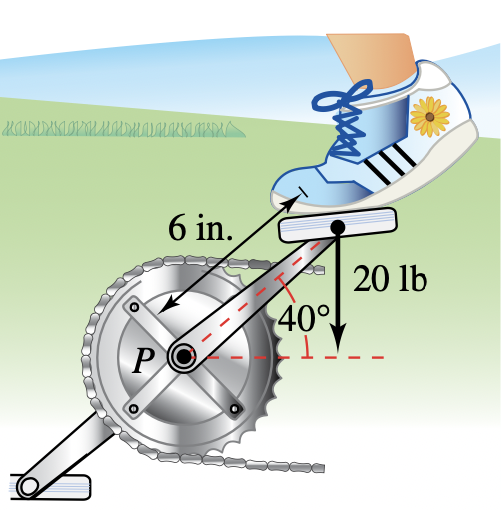
\includegraphics[scale=0.55]{assets/larson11.4q27.png}
          \end{center}
          \newpage
          \sol{} Let the force $\vec{F} = \langle 0, 0, -100 \rangle$ and the position vector of the pedal $\vec{r} = \langle 0, 0.17\cos40^{\circ}, 0.17\sin40^{\circ} \rangle$.
          \begin{align*}
              \vec{\tau}        & = \vec{r} \times \vec{F}                                                                   \\
                                & = \begin{vmatrix}
                                        \hat{\imath} & \hat{\jmath}       & \hat{k}            \\
                                        0            & 0.17\cos40^{\circ} & 0.17\sin40^{\circ} \\
                                        0            & 0                  & -100
                                    \end{vmatrix}               \\
                                & = \hat{\imath} \begin{vmatrix}
                                                     0.17\cos40^{\circ} & 0.17\sin40^{\circ} \\
                                                     0                  & -100
                                                 \end{vmatrix} - \hat{\jmath} \begin{vmatrix}
                                                                                  0 & 0.17\sin40^{\circ} \\
                                                                                  0 & -100
                                                                              \end{vmatrix} + \hat{k} \begin{vmatrix}
                                                                                                          0 & 0.17\cos40^{\circ} \\
                                                                                                          0 & 0
                                                                                                      \end{vmatrix} \\
                                & = \hat{\imath}(-17\cos40^{\circ}) - \hat{\jmath}(0) + \hat{k}(0)                           \\
                                & = \langle -17\cos40^{\circ}, 0, 0 \rangle                                                  \\
              \norm{\vec{\tau}} & = \sqrt{(-17\cos40^{\circ})^2 + 0^2 + 0^2} = 17\cos40^{\circ} \approx 13.023 \text{ J}
          \end{align*}
          $\hfill\blacksquare$
          \setcounter{enumi}{28}
    \item \textbf{Optimization} A force of 180 newtons acts on the bracket shown in the figure.
          \begin{center}
              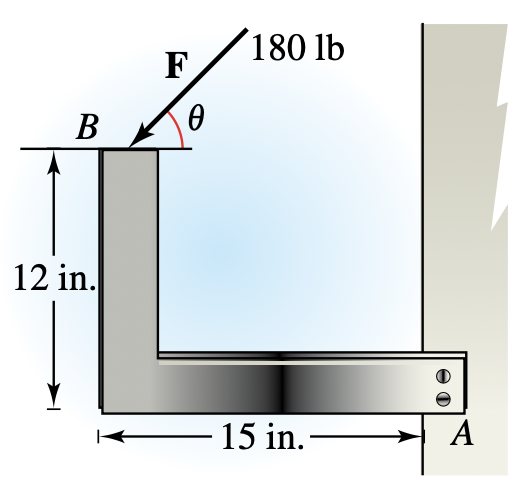
\includegraphics[scale=0.55]{assets/larson11.4q29.png}
          \end{center}
          \begin{enumerate}[label={(\alph{*})}]
              \item Determine the vector $\overrightarrow{A B}$ and the vector $\mathbf{F}$
                    representing the force. ( $\mathbf{F}$ will be in terms of $\theta$.) \sol{}
                    The horizontal and vertical distances between $A$ and $B$ are $-40$cm and
                    $32$cm respectively. Hence, $\overrightarrow{A B} = -0.4j + 0.32k$.
                    $\hfill\blacksquare$ \newpage
              \item Find the magnitude of the moment about $A$ by evaluating $\|\overrightarrow{A
                            B} \times \mathbf{F}\|$. \sol{}
                    \begin{align*}
                        \overrightarrow{A B} \times \mathbf{F}        & = \begin{vmatrix}
                                                                              \hat{\imath} & \hat{\jmath}   & \hat{k}        \\
                                                                              0            & -0.4           & 0.32           \\
                                                                              0            & -180\cos\theta & -180\sin\theta
                                                                          \end{vmatrix}                   \\
                                                                      & = \hat{\imath} \begin{vmatrix}
                                                                                           -0.4           & 0.32           \\
                                                                                           -180\cos\theta & -180\sin\theta
                                                                                       \end{vmatrix} - \hat{\jmath} \begin{vmatrix}
                                                                                                                        0 & 0.32           \\
                                                                                                                        0 & -180\sin\theta
                                                                                                                    \end{vmatrix} + \hat{k} \begin{vmatrix}
                                                                                                                                                0 & -0.4           \\
                                                                                                                                                0 & -180\cos\theta
                                                                                                                                            \end{vmatrix} \\
                                                                      & = \hat{\imath}(72\sin\theta + 57.6\cos\theta) - \hat{\jmath}(0) + \hat{k}(0)           \\
                                                                      & = \langle 72\sin\theta + 57.6\cos\theta, 0, 0 \rangle                                  \\
                        \\
                        \norm{\overrightarrow{A B} \times \mathbf{F}} & = \sqrt{(72\sin\theta  57.6\cos\theta)^2 + 0^2 + 0^2}                                  \\
                                                                      & = |72\sin\theta + 57.6\cos\theta|
                    \end{align*}
                    $\hfill\blacksquare$
              \item Use the result of part (b) to determine the magnitude of the moment when
                    $\theta=30^{\circ}$. \sol{} When $\theta=30^{\circ}$, \[\norm{\overrightarrow{A B} \times \mathbf{F}} = |72\sin30^{\circ} + 57.6\cos30^{\circ}| = 85.883 \text{ J}\]

              \item Use the result of part (b) to determine the angle $\theta$ when the magnitude
                    of the moment is maximum. At that angle, what is the relationship between the
                    vectors $\mathbf{F}$ and $\overrightarrow{A B}$ ?
                    $\dfrac{d}{d\theta}(|72\sin\theta + 57.6\cos\theta|) = 0$. Hence,
                    \begin{align*}
                        \dfrac{d}{d\theta}(|72\sin\theta + 57.6\cos\theta|) = \dfrac{72\cos\theta - 57.6\sin\theta}{|72\sin\theta + 57.6\cos\theta|} & = 0                                                         \\
                        72\cos\theta                                                                                                                 & = 57.6\sin\theta                                            \\
                        \tan\theta                                                                                                                   & = \dfrac{72}{57.6} = \dfrac{5}{4}                           \\
                        \theta                                                                                                                       & = \tan^{-1}\left(\dfrac{5}{4}\right) \approx 51.340^{\circ} \\
                        F \cdot \overrightarrow{A B}                                                                                                 & = 180\cos\theta \times -0.4 + 180\sin\theta \times 0.32     \\
                                                                                                                                                     & = -72\cos
                    \end{align*}
                    When $\theta = 51.340^{\circ}$, $\mathbf{F}$ and $\overrightarrow{A B}$ are perpendicular to each other. $\hfill\blacksquare$
          \end{enumerate}
\end{enumerate}